\documentclass[PI,LAB]{HSEUniversity}

\usepackage{graphicx}
\graphicspath{ {img/} }

\usepackage{hyperref}
\hypersetup{
    colorlinks=true,
    linkcolor=black,
    filecolor=magenta,      
    urlcolor=cyan,
}

\title{Организация паттернов проектирования. Структурный паттерн <<Заместитель>>}
\author{Рязанов Иван Дмитриевич}
\supervisor{к.т.н., доцент кафедры Информационных технологий в бизнесе НИУ ВШЭ-Пермь}{А.В.~Кычкин}
\Year{2020}

\begin{document}
\maketitle
\chapter{Паттерн <<Заместитель>>}
\textbf{Название и классификация паттерна.}
Заместитель - паттерн, структурирующий объекты, который предоставляет объект, который контролирует доступ к другому объекту, перехватывая все вызовы.

\textbf{Назначение.}
Управление ресурсоемкими объектами, при котором нет необходимости создавать экземпляры таких объектов до момента их реального использования. Proxy является суррогатом другого объекта и управляет доступом к нему.

Заместитель это объект, интерфейс которого идентичен интерфейсу реального объекта. При первом запросе клиента заместитель создает реальный объект, сохраняет его адрес и затем отправляет запрос этому реальному объекту. Все последующие запросы просто переадресуются инкапсулированному реальному объекту.

\textbf{Применимость.}
Существуют ситуации, когда можно использовать паттерн Proxy:
\begin{enumerate}
	\item Виртуальный proxy является заместителем объектов, создание которых обходится дорого. Реальный объект создается только при первом запросе/доступе клиента к объекту. 
	\item Удаленный proxy предоставляет локального представителя для объекта, который находится в другом адресном пространстве. 
	\item Защитный proxy контролирует доступ к основному объекту. "Суррогатный" объект предоставляет доступ к реальному объекту, только вызывающий объект имеет соответствующие права.
	\item Интеллектуальный proxy выполняет дополнительные действия при доступе к объекту.
\end{enumerate}
\clearpage

\begin{figure}[p]
  \centering
  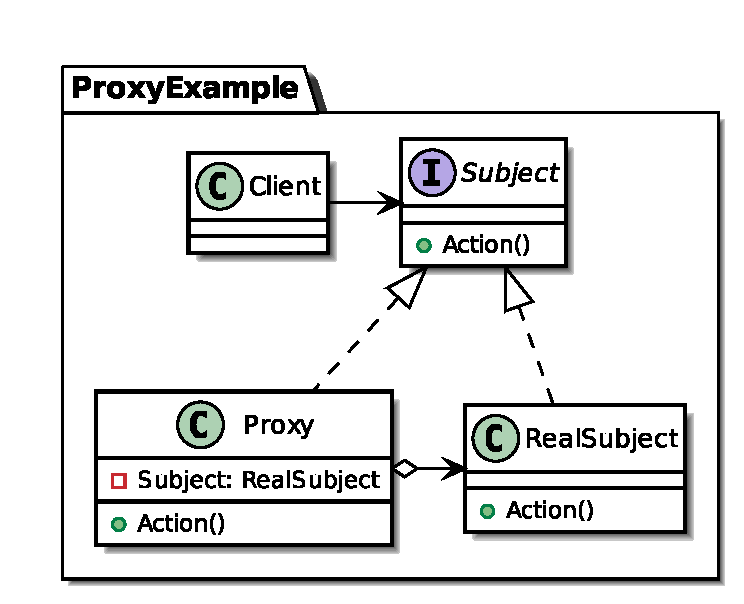
\includegraphics[scale=0.7]{Proxy_CD.eps}
  \caption{Диаграмма классов паттерна <<Заместитель>>}
\end{figure}

\begin{figure}[p]
  \centering
  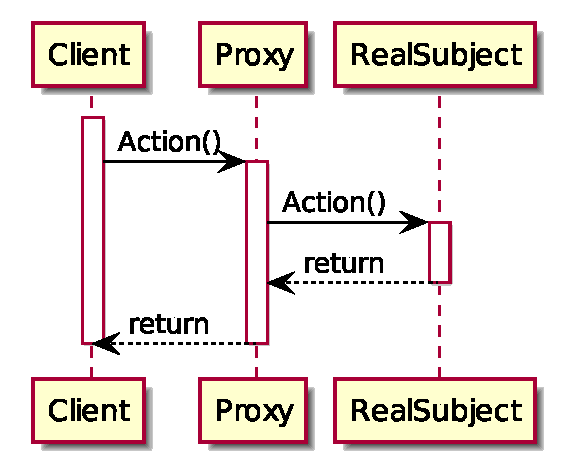
\includegraphics[scale=0.75]{Proxy_SD.eps}
  \caption{Диаграмма последовательности паттерна <<Заместитель>>}
\end{figure}
\clearpage

\textbf{Участники}

\begin{enumerate}
	\item Proxy - заместитель:
	\begin{itemize}
		\item хранит ссылку, которая позволяет заместителю обратиться к реальному субъекту. Объект класса Proxy может обращаться к объекту класса Subject, если интерфейсы классов RealSubject и Subject одинаковы;
		\item предоставляет интерфейс, идентичный интерфейсу Subject, так что заместитель всегда может быть подставлен вместо реального субъекта;
		\item контролирует доступ к реальному субъекту и может отвечать за его создание и удаление;
		\item прочие обязанности зависят от вида заместителя:
		\item \textit{удаленный заместитель} отвечает за кодирование запроса и его аргументов и отправление закодированного запроса реальному субъекту в другом адресном пространстве;
		\item \textit{виртуальный заместитель} может кэшировать дополнительную информацию о реальном субъекте, чтобы отложить его создание. 
		\item \textit{защищающий заместитель} проверяет, имеет ли вызывающий объект необходимые для выполнения запроса права;
	\end{itemize}
	\item Subject - субъект: определяет общий для RealSubject и Proxy интерфейс, так что класс Proxy можно использовать везде, где ожидается RealSubject;
	\item RealSubject - реальный субъект: определяет реальный объект, представленный заместителем.
\end{enumerate}

\textbf{Отношения}
Proxy при необходимости переадресует запросы объекту RealSubject. Детали зависят от вида заместителя.

\textbf{Плюсы и минусы}
Плюсы:
\begin{enumerate}
	\item Позволяет контролировать сервисный объект незаметно для клиента.
	\item Может работать, даже если сервисный объект ещё не создан.
	\item Может контролировать жизненный цикл служебного объекта.
\end{enumerate}

Минусы:
\begin{enumerate}
	\item Усложняет код программы из-за введения дополнительных классов. 
	\item Увеличивает время отклика от сервиса.
\end{enumerate}

\textbf{Области применения}

\begin{enumerate}
	\item Системы доставки контента (кеширование важно).
	\item ПО, требующее авторизацию пользователей.
\end{enumerate}

\chapter{Проектирование и реализация}
\section{Проектирование}
Для реализации был выбран 3 вариант:

<<Программа для обеспечения оплаты подписок на сервисы.>>

 \begin{figure}[h]
   \centering
   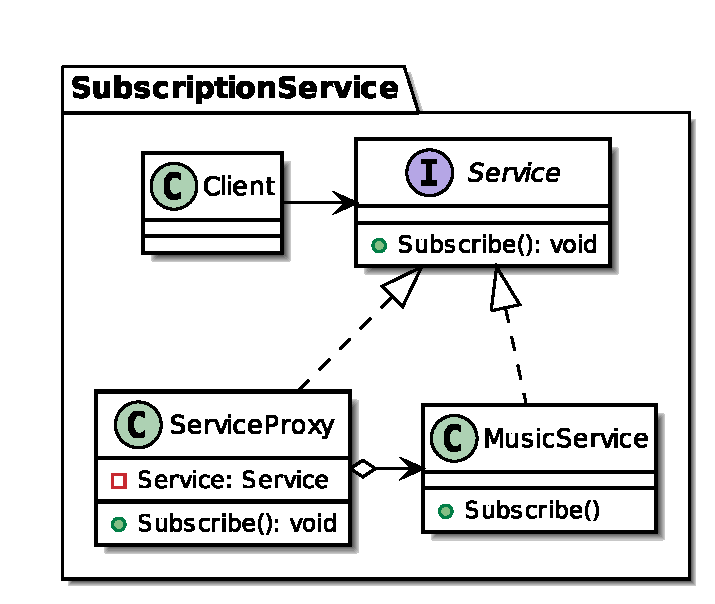
\includegraphics[scale=0.75]{Task_CD.eps}
   \caption{Диаграмма классов}
   \label{fig:Task_CD}
 \end{figure}

\textbf{Участники}

\begin{enumerate}
	\item Service --- сервис, на который можно подписаться.
	\item MusicService --- реализация сервиса в виде сервиса предоставления музыки.
	\item ServiceProxy --- заместитель, который контролирует оплату перед подпиской на сервис.
	\item Client --- клиентская часть программы.
\end{enumerate}

\section{Реализация}
Реализация паттерна <<Заместитель>> находится в git-репозитории по ссылке: \href{https://github.com/rovany706/design-patterns/}{github.com}

\end{document}
